\begin{figure}[h]
  \centering
  \begin{tabular}{ p{6cm} p{6cm} }
    \centering 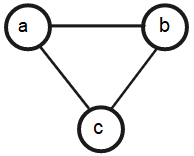
\includegraphics[width=2.3cm]{./img/trianguloabc.png} & 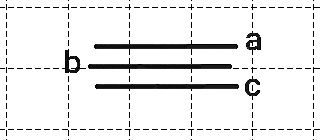
\includegraphics[width=3.5cm]{./img/b0epgTransparenciaGrade2.png}
    \\
    \footnotesize \centering (a) The  graph $C_3$ & \footnotesize(b) $B_0$-EPG representation of $C_3$  \\
&  \\ \centering
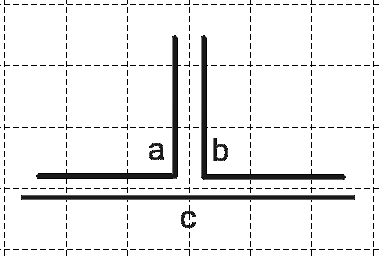
\includegraphics[width=3.5cm]{./img/b1EpgTransparenteGrade2.png} %b1epgtriangulo
     & 
  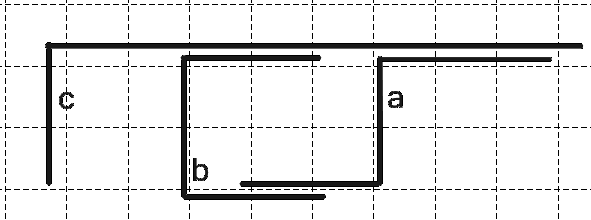
\includegraphics[width=5cm]{./img/b2epgTransparenciaGrade2.png}\\
  \footnotesize \centering (c) $B_1$-EPG representation of $C_3$  &  \footnotesize  (d) $B_2$-EPG representation of $C_3$ \\
  \end{tabular}

 \caption{The  graph $ C_3 $  and some representations: without bends, with 1 bend and with 2 bends} \label{fig:trianguloepgRepresentacao}
\end{figure}